\documentclass{standalone}
\usepackage{tikz}
\usepackage{ctex,siunitx}
\setCJKmainfont{Noto Serif CJK SC}
\usepackage{tkz-euclide}
\usepackage{amsmath,mhchem}
\usetikzlibrary{patterns, calc}
\usetikzlibrary {decorations.pathmorphing, decorations.pathreplacing, decorations.shapes,}
\begin{document}
\small
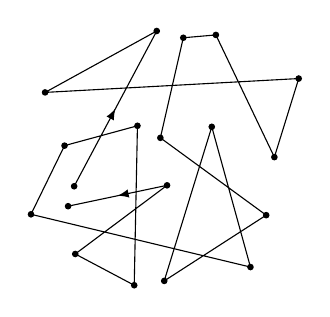
\begin{tikzpicture}[>=latex,scale=1.0]
  \draw(0.750,1.478)--(1.799,3.450)--(0.381,2.670)--(3.602,2.846)--(3.293,1.848)--(2.550,3.400)--(2.136,3.364)--(1.845,2.093)--(3.189,1.111)--(1.894,0.276)--(2.498,2.233)--(2.989,0.452)--(0.202,1.122)--(0.628,1.994)--(1.554,2.246)--(1.513,0.221)--(0.764,0.618)--(1.930,1.490)--(0.673,1.225);
  \draw[decorate,decoration={markings,mark=at position 0.5 with {\arrow{>}}}](0.750,1.478)--(1.799,3.450);
  \draw[decorate,decoration={markings,mark=at position 0.5 with {\arrow{>}}}](1.930,1.490)--(0.673,1.225);
  \foreach \x/\y in {0.750/1.478,1.799/3.450,0.381/2.670,3.602/2.846,3.293/1.848,2.550/3.400,2.136/3.364,1.845/2.093,3.189/1.111,1.894/0.276,2.498/2.233,2.989/0.452,0.202/1.122,0.628/1.994,1.554/2.246,1.513/0.221,0.764/0.618,1.930/1.490,0.673/1.225}
  {\fill(\x,\y)circle(1.2pt);}
\end{tikzpicture}
\end{document}